\documentclass{article}
\usepackage[utf8]{inputenc}
\usepackage{natbib} % For cites and references
\bibstyle{apalike} % Apa style of bibliography
\usepackage{titlesec} % for the paragraphs
%% Copy pasted from internet
\usepackage{hyperref} % for the hyperlinks
\usepackage{hologo} % for the bibtex logo
\usepackage{graphicx} %for the images
\usepackage{nameref} %to make appear the name instead of number when referring to a section

\usepackage{wasysym}

%\usepackage{amssymb}% for the ↹  symbol

\usepackage{pdflscape} % To leave pages in landscape
\usepackage{everypage} % To make the number stay down in the landscape page
\usepackage{lipsum} % To make number stay down in landscape page 

%% https://tex.stackexchange.com/questions/278113/single-landscape-page-with-page-number-at-the-bottom
% QUe lo haga sara

\setcounter{secnumdepth}{4}
\titleformat{\paragraph}
{\normalfont\normalsize\bfseries}{\theparagraph}{1em}{}
\titlespacing{\paragraph}
{0pt}{3.25ex plus 1ex minus .2ex}{1.5ex plus .2ex}
%%

\bibliographystyle{apalike}

\title{Guide for Ph.D.s}
\author{Carlos Alcala }
\date{February 2020}

\begin{document}

\maketitle
\tableofcontents

\subsection{Introduction}
\label{subsec: intro}
Welcome!

I am writing this guide as a small help and document of reference along your path as a Ph.D student at the IPSY institute of UCLouvain. 

In case you are a research assistant or an intern, this guide can also help you. Thus, first of all, get to know your status and the characteristic of your enrollment in the institute. You may have to follow different procedures. 

I start writing in a Word file, and then I typeset the guide using \href{https://www.overleaf.com/}{Overleaf}, an online \href{https://www.latex-project.org/}{\LaTeX} editor. Also, I thought about transform it into a \href{https://bookdown.org/}{Bookdown} \citep{xie2016bookdown}, or making a \href{https://github.com/}{GitHub} project. But time is not allowing me to do all these things. So for the moment, you will have to feel satisfied with this.

I also wrote this guide thinking in a collaborative project where people could comment and update the information according to the changes of time. For that, tools like \href{https://github.com/}{GitHub} or \href{https://web.hypothes.is/}{Hypothes.is} seem the most suitable for me. Therefore, if you are interested in the original text, to be able to make modifications, don't hesitate in sending me an email at \href{mailto: carlos.alcala@ucluvain.be}{carlos.alcala@ucluvain.be} or \href{mailto: carlitofluito@gmail.com}{carlitofluito@gmail.com}.


\section{Fundamentals}
\label{sec:Fundament}
\subsection{Developing a \textsc{system}: organization and registration}
\label{subsec: System}

I have an \textsc{adhd} brain. One of the things that the people with our type of brains needs and love the most is structure and organization. Usually, one that works for our type of mind, one that we agree with. We don’t like imposed rules that we have to follow, but we are very thankful of systems that help us keep our mind in order. Consider the tons of ideas that our brains constantly generate, and how difficult can be to allocate them in a place where we can later find them. You may find my folder-sub folder tendency excessive, but it works for me. And it may work for you…

Using a good and effective system will save you tons of frustration and lost time looking files up and down. Usually, you develop one that suits your needs by trial and error. You can update yours with time, year after year, improving in what it previously didn't work, and adding aspects you didn't predict.

The system may generate duplicates, like adding the same paper to different topics in the \textsc{literature} folder, or duplicating graphs in the \textsc{manuscript} and \textsc{data} folder. 

Also, a key aspect of a Ph.D. is to register pretty much everything you do since the first steps. Doing this will help your memory when you want to recall what exactly did you do to get some results, or which specific items of the scale did you use.

In my case this is an approximation of my system: 

\begin{landscape}
\begin{figure}
\centering
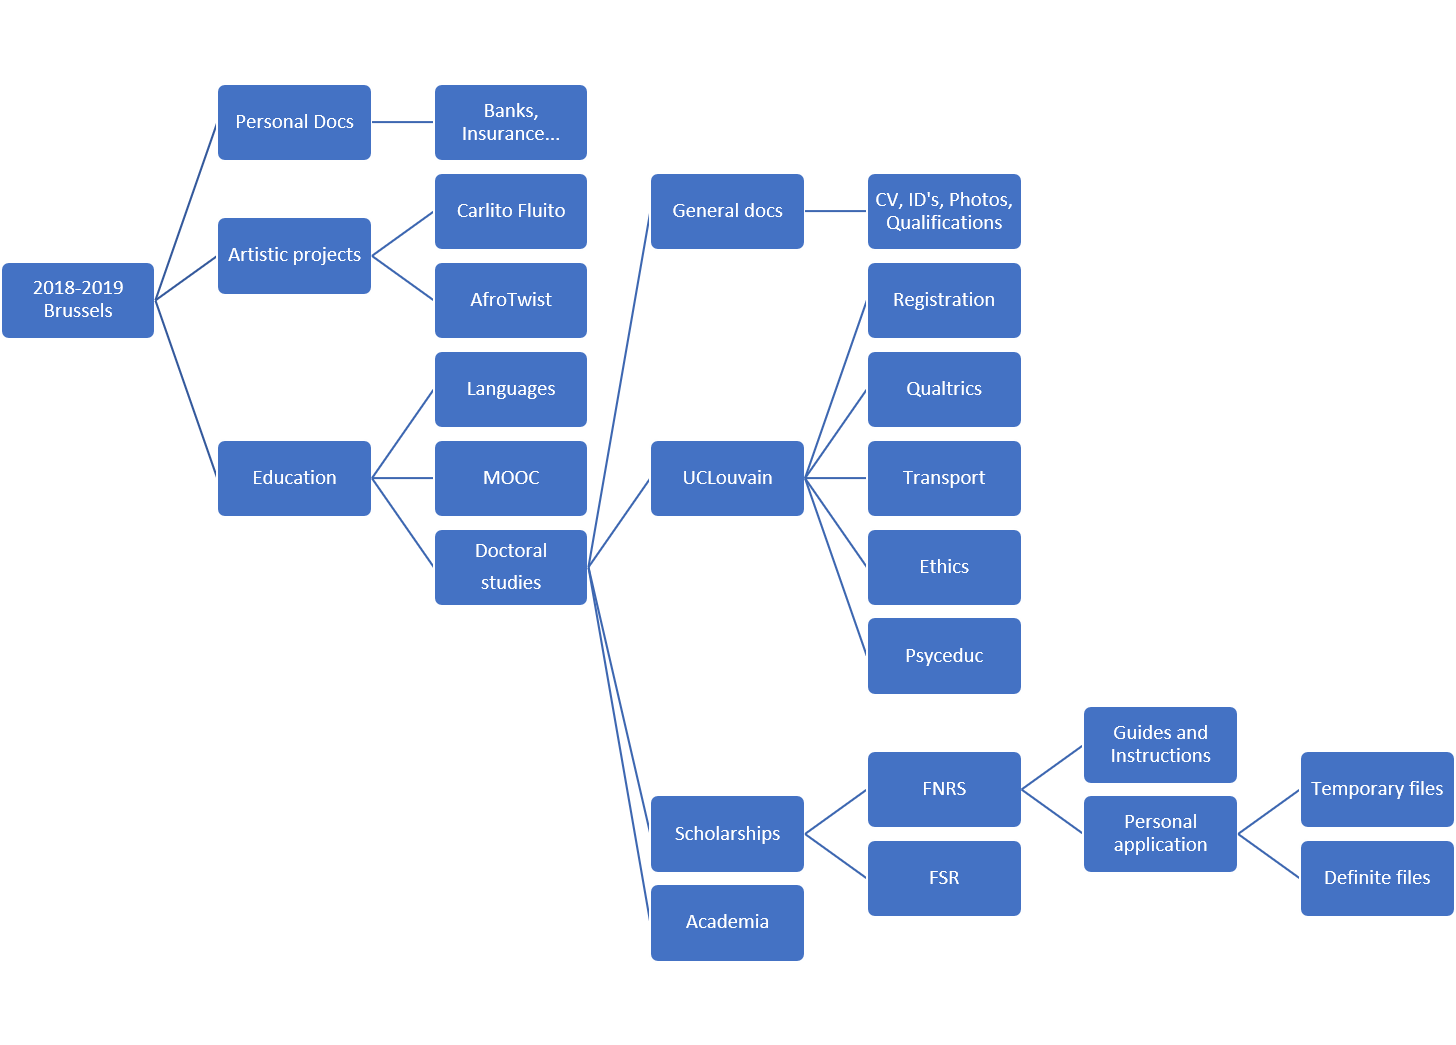
\includegraphics[height = 0.75\textwidth]{images/tree1.png}
\caption{A tree of my folders.}
\label{fig: tree1}
\end{figure}
\end{landscape}

\subsubsection{ORGANIZATION: Folders, sub-folders, files and sub-files in your laptop}
\label{subsubsec: organization}

\paragraph{Naming files}
\label{parag: naming}

To start with, get use to set up the name of your files (folders and projects) with the date at the beginning in the format \textsc{yyyy-mm-dd}. This way all files and folders get ordered chronologically and automatically. Also, it is a great way to have the latest version easily accessible when you are working on a file and making modifications. It can be a bit annoying and repetitive and platforms and tools like \href{https://www.google.com/docs/about/}{Google Docs}, \href{https://www.latex-project.org/}{\LaTeX}, \href{https://en.wikipedia.org/wiki/Markdown}{Markdown}, \href{https://github.com/}{GitHub} branches, \href{https://web.hypothes.is/}{Hypothes.is}, or an online text editor with comments can help much of this type of mess. However, learning some of these tools takes times and sometimes advisors are not very willing to update themselves. Try to push the change, but anyway, it is worthwhile to learn it for your own future projects. 

\paragraph{Year by year}
\label{parag: year}

Each year/scholar course, I create a new folder with the number of the year and the city I was living in. 

For example: 
\begin{center}
\textsc{2018-2019 Brussels}
\textsc{2019-2020 Brussels}
\end{center}

\paragraph{By life topic}
\label{parag: topic}
Inside each year, I make different folders for different areas and occupations of my life: 
\begin{center}
  \textsc{personal docs} 
\end{center}
Here I keep official docs, banks and insurance paper, etc.\footnote{If you are a hacker wanting to screw me up, you can find lot of personal information here. Please, don’t. I am just a simple nice guy trying to make the world a better place. Thanks!}
\begin{center}
   \textsc{artistic projects}
\end{center}
I am leaving my Ph.D. studies to become a full-time artist (a dancer). So, I need this folder for all the creative works going on.
\begin{center}
    \textsc{education}
\end{center}
In \textsc{education}, I may have other things apart from the \textsc{doctoral studies}, such as online courses (\textsc{MOOC}\footnote{\href{ https://www.mooc.org/}{Massive Open Online Courses}. It is 2020, and you can learn \textsc{anything} and \textsc{everything} online. High quality intellectual information can be found from the internet if you know some reliable sources. Click on any of the following words: \href{https://www.edx.org/}{EdX}, \href{https://www.coursera.org/}{Coursera}, \href{https://www.datacamp.com/}{DataCamp}, \href{https://www.udemy.com/}{Udemy}, \href{https://www.duolingo.com/}{DuoLingo}, \href{https://miriadax.net/home}{MiriadaX}. My CV has significantly increase thanks to this. Give it a chance.}), or language courses. Since this is a guide for Doctoral studies, we will focus on the \textsc{education} folder.

\paragraph{Doctoral studies}
\label{parag: doct}
In the \textsc{education} folder, I create the \textsc{doctoral studies}  folder for academic and university files. There, I divide between paperwork and official procedures and pure academic work. 
\begin{center}
    \textsc{general docs}
\end{center}
In \textsc{general docs}, I have titles, qualifications, CV’s, portrait picture, ID copies and other files that I may need in future applications, scholarships, etc. Easy to access.\footnote{Here, I can have duplicates with the PERSONAL DOCS folder, but I don’t mind. I want easy and quick access when I am applying for a scholarship or renewing my registration at the university office.}
\begin{center}
    \textsc{UCLouvain}
\end{center}
In \textsc{UCLouvain}, I have a folder for the \textsc{cdd}\footnote{Comission Doctorale}, \textsc{qualtrics} (files and procedure of activation), \textsc{registration} (university paperwork), \textsc{transport}, \textsc{ethics}\footnote{You may need to have an \textsc{ETHICS} folder in each of your studies, in case you have to write several Ethical protocols.}  (Ethical committee approval), \textsc{psyceduc}\footnote{I have left the section \nameref{subsec: PSYCEDUC} unwritten. The enroll process can can be a bit complicate to get around. Feel free of adding it to this guide and erase this footnote.} courses, etc. Mostly paperwork of the university.
\begin{center}
    \textsc{scholarships}
\end{center}
In \textsc{scholarships}, I have the different scholarships I apply. For example, \textsc{fnrs} has \textsc{guides and instructions}, and \textsc{personal application}. I advise you to keep the ``\textsc{yyyy-mm-dd}'' to keep it organized. Eventually, make two folders called: \textsc{temporary files}, to put the files and temporary applications; and \textsc{definitive files}, to put the definite application that you have sent. 

\emph{Pro advice}. Move the files to the \textsc{definitive files} at the moment of sending them, so you don’t mess up making changes, or having the classical “Definitive Version 3 changed, corrected, updated and reviewed”. The \textsc{definitive files} folder is to know what you send in the future, when you need to retrieve the application.
\begin{center}
    \textsc{academia}
\end{center}
This gets complicated…

\begin{landscape}
\begin{figure}
\centering
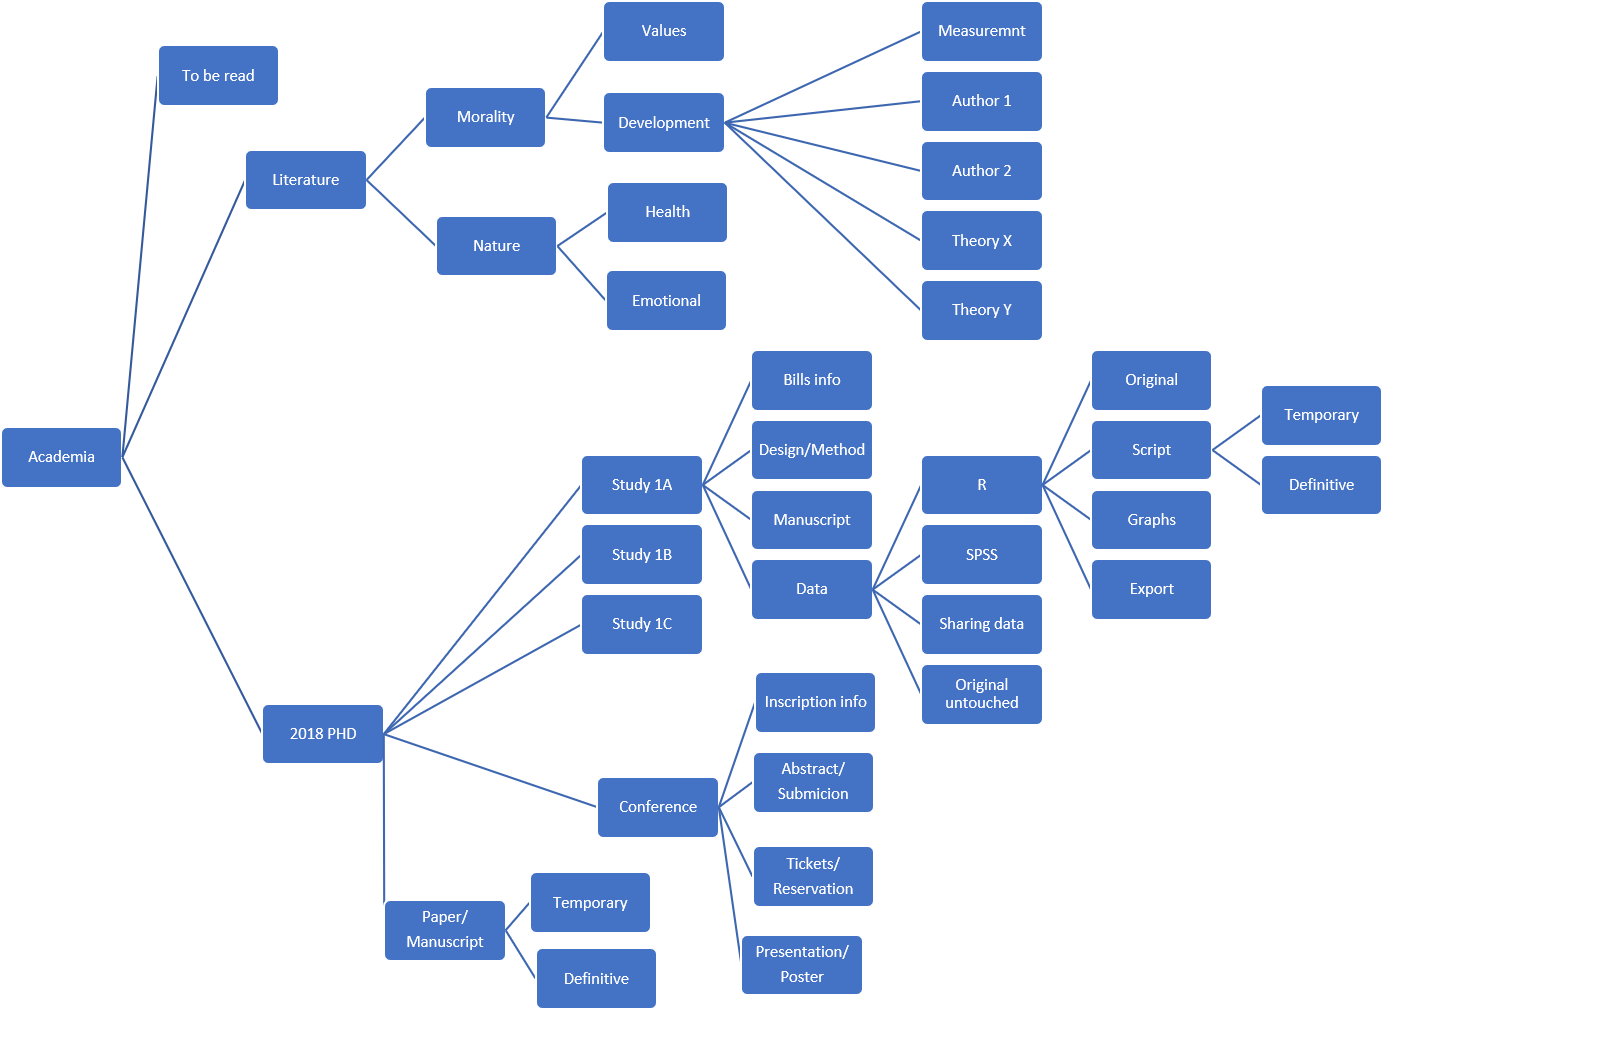
\includegraphics[height = 0.75\textwidth]{images/tree2.png}
\caption{A tree of my folders inside the academia folder.}
\label{fig: tree2}
\end{figure}
\end{landscape}


\paragraph{Academia}
\label{parag: Acad}
\textsc{academia} folder can get a bit of a mess. It is important that you find a structure that works for you. In my case, I have several folders: 
\begin{center}
    \textsc{to be read}
\end{center}
It is a sort of ``\textsc{future readings}'' folder. If you keep yourself updated, you may want to check known journals from time to time (Once a month sounds good). You may find interesting stuff that you don’t know where to allocate, or that relates to several topics that are not your main field of research. In this case, you can use this folder to leave these types of things. In the best of the cases, you can make a PowerPoint (Check \nameref{subsubsec: Registr}), to keep your findings sort of ordered and under control. Checking the abstract and add it to the PowerPoint should be okay. 

I also advice to review this folder once a month (I know, it may never happen). You can try to sort them out, make new folders in the \textsc{literature} or new research projects beyond your PHD.  

\emph{Pro advice}. You may want to have a proper naming system for your journals. It is horrendous to open a folder full of paper and find indecipherable characters that came as a default name when you download the PDF files. Get used to name all files as soon as possible (at the moment of download) in a way that is understandable. More on this on \nameref{parag: literat} and the \nameref{subsec: shortcut} sections.
\begin{center}
    \textsc{literature}
\end{center}

My advice is that you keep this as organized as possible. In my case, I have many folders that can became sub-folders. My Ph.D. used to be about Moral effects of exposure to nature.

Thus, I had a folder named \textsc{morality}  with sub-folders of different theories like \textsc{moral development}, \textsc{values}, \textsc{moral emotions}…. Inside each of these, I could make a sub-folder of \textsc{measurements}, another with some specific \textsc{authors} that are very relevant, or with some specific \textsc{theories} concerning the field.

I also have another folder of \textsc{nature}, where I decided to aggregate the papers concerning their different effects in \textsc{emotions}, \textsc{health}, \textsc{behavior}… In each of these, I might have created \textsc{author}, \textsc{theories}, and \textsc{measurements} folders.

A very important detail is to save the papers with a coherent naming system. In my case, each PDF file is names as 
``\textsc{yyyy} Author, author - Key words of title''. Observe the names of the files in figure \ref{fig: papers}\footnote{You can notice that the path is not the same as I describe in the guide. It took me some time and refinement to get to where I explain here. It may not be the definitive version, since I may update and improve it in the future.}: 

\begin{figure}
\centering
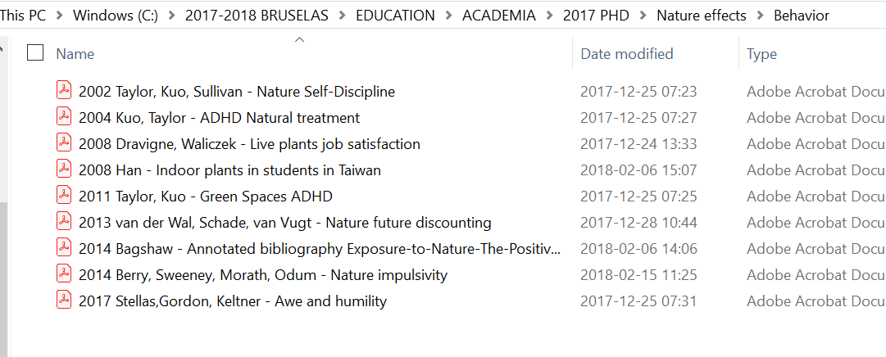
\includegraphics[width = \textwidth]{images/papers.png}
\caption{A screenshot of one of my folders.}
\label{fig: papers}
\end{figure}

This way, I have easy and quick access to original papers whenever I need them. Another key tool for keeping your literature handy and useful is to work with the Power Points. (Check section \nameref{subsubsec: Registr}).

\paragraph{YYYY Ph.D.}
\label{parag: YYYY}

Here you can save the main activities concerning a Ph.D.: the design and carrying out of studies, your participation in conferences, and the manuscript you prepare for submission. 

The \textsc{conferences} folder can have different sub-folders for each conference. Within these, you can create sub-folders with \textsc{inscription info, tickets/reservation, abstract/submission, presentation/poster} to keep things handy for the future (as in updating your \textsc{CV} or knowing what exactly you presented).

Also, you can make a folder called \textsc{yyyy-mm manuscript} to keep the files concerning the writing of the manuscript, especially if you are including different studies (experiments) in one paper. This folder can get messy as well, remember to name everything as “yyyy-mm-dd” to keep the order. However, if you can learn \href{https://crsh.github.io/papaja_man/}{\textsc{papaja} package}  in R, and write the whole manuscript, you may save tons of organizing and duplicating files. Also, leaning \href{https://www.latex-project.org/}{\LaTeX} and using Overleaf can be a good investment.

In the folder \textsc{studies}, I made a sub folder for each of the studies that I run along the year (mostly experimental in my case). As you can see in the figure \ref{fig: folders} \footnote{In the same way, I have a slightly different path, and I haven’t sub-divided this folder in \textsc{studies, conference,} and \textsc{manuscript}. Looks okay, but a bit messy for my taste.}, I keep a system for naming the studies:
\begin{center}
    \textsc{yyyy-mm} key words - \textsc{key code} (number-letter) 
\end{center}

In the code (\textsc{1A, 1B, 1C}), I refer to the year of Ph.D. that I run the study (1 for the first year, 2 for the second); and the letter as the order in which I do the studies (A for the first; B the second). You can also choose a strictly numeric system (1.1, 1.2; 2.2), but I am not so good at seeing numbers and it can be confusing. Your choice, anyways. 

\begin{figure}
\centering

\includegraphics[width = \textwidth]{images/folders.png}
\caption{A screenshot of the folders of my studies.}
\label{fig: folders}
\end{figure}

\paragraph{Studies}
\label{parag: studies}
Within each study folder, I have 
\begin{center}
    \textsc{bills info}
\end{center}

I can keep the bills (if I pay participants, buy some materials, or the online platform). Useful when you want to recover your money and have to send bills to the finance office. (Check the How to get refunded section)
\begin{center}
    \textsc{design – methodology}
\end{center}

Here I save the original material I am using for the study and the procedure: Pictures, measurements and questionnaires, a word file explaining the design of the study with the full references. Also, it is recommendable to make a \textsc{temporary files} and \textsc{definitive files} folders with the ones you end up using, since you are likely to make modification and adjustments along the designing process. 
\begin{center}
    \textsc{manuscript}
\end{center}

Since it is divided by studies, here you can keep the \emph{Method and results} section of the study. You can use the \textsc{yyyy-mm} Manuscript folder for the main writing process.

\paragraph{Data and R project}
\label{parag: Data}
I partly applied the organizational strategy presented in the \href{https://bookdown.org/ndphillips/YaRrr/importingdata.html}{\textsc{yarrr} book, chapter 9} \footnote{More info in the \nameref{subsec: learn R} section below}. I adapted his suggestions to my needs and knowledge. It took me some time and exploration but following this and the \textsc{yarrr} guide can be a good starting point.
\begin{center}
    \textsc{data}
\end{center}
This folder is pretty important. In my case, I have different sub folders:
\begin{center}
    \textsc{original untouched}
\end{center}
The data set as downloaded in \href{https://www.qualtrics.com/uk/?rid=ip&prevsite=en&newsite=uk&geo=DE&geomatch=uk}{Qualtrics}. No modifications. You can also save a survey example filled by a participant, the last version of your survey/experiment, or whatever final procedure you use.
\begin{center}
    \textsc{sharing data}
\end{center}
You may have many working files with different including/excluding criteria, outlier participants, different models, explorations, subgroups, etc.… However, at some point you will have to make decisions and move forwards. Therefore, after many modifications and changes, you will end up having a final dataset that you use for your official results, sharing with your advisor when you leave and finish, checking numbers while writing your dissertation, or sharing with other researchers and reviewers. Keep it clean, readable and understandable for a third person. Save it here with the name “yyyy-mm-dd Study 1A sharing data”. You may want to make a copy with a name for a third person “Surname, name (\textsc{yyyy}) Manuscript Name. Study 1”. 
\begin{center}
    \textsc{spss}
\end{center}
Here I have \emph{.sav} files with the working dataset. I am not worrying much about modifications, although it is clear the problem of duplicating files with slight changes that you can avoid by using R.
\begin{center}
    \textsc{r}
\end{center}
R with sub folders names \textsc{graphs, script, original}, and \textsc{export}. This is depending on my working flow. Usually, I write an R script (in the \textsc{script} folder). With this script, I import the data from the \textsc{original}L folder (copied from untouched data), and I export the modified data in the \textsc{export} folder as an .sav file to work on \textsc{spss} with my advisor (\href{https://www.rdocumentation.org/packages/haven/versions/2.2.0}{\emph{haven} package}). In the \textsc{graphs} folder, I export the graphs and visualizations (\href{https://ggplot2.tidyverse.org/}{\emph{ggplot}}\citep{wickham2007ggplot} and \href{https://purrr.tidyverse.org/}{\emph{purrr}}\citep{henry2017purrr} packages). I can make a \textsc{temporary} and \textsc{definitive} folder here as well for quickly accessing to the last version, or once the analysis are done.

\subsubsection{REGISTRATION: The Power of PowerPoint}
\label{subsubsec: Registr}
Something I realized a bit late but that could have saved hours of duplicated work, repeated searches, and organization was an alternative usage of Power Points. In my case, I use Power Points not only for presentations but as organization method. There are two principal usages: 

\paragraph{Organizing your literature}
\label{parag: literat}
The first usage resembles an old school library catalog made of cards. In the folder of the topic of your literature you can create:
\begin{itemize}
    \item a PDF file with the search of the PyscInfo (or another database where you get the literature), 
    \item a DOC file with the information you use (key words, date, database, why are you making the search), and,
    \item PowerPoint with the main findings. 
\end{itemize}

For the PowerPoint, I do the following. I put all the basic information of one paper in one slide, and then I order them chronologically, from the newest to the oldest. The title of the slide is the full reference, and with bullet points, I write down a bit of methodology and results. In the figure \ref{fig: Powerpoint} you can see few articles concerning the ``Four immeasurable'', Buddhist concept. The literature is not so big (for the moment), so I can have all the existing literature available in one PowerPoint file. That is very handy.
\begin{center}
\begin{figure}
    \centering
    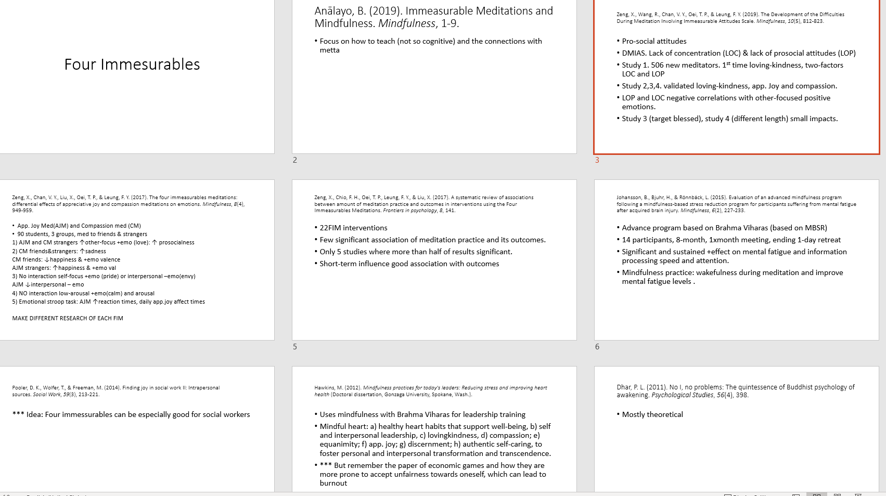
\includegraphics[width = 0.75\textwidth]{images/ppt.png}
    \caption{A screenshot of one of my Power Points of a literature review }
    \label{fig: Powerpoint}
\end{figure}
\end{center}
This way, I can move quickly among the literature of a certain topic and I find the information fast. Also, if you have a vague memory of a paper you once read, but you forgot about whether you download it or not, or where you saved it, you can quickly find the information if you registered it in the PowerPoint. Even further, PowerPoint allows you to make sections, and move and copy slides. Therefore, you can include new papers at any moment in different PowerPoint’s concerning to a certain topic. In a similar way, it is not problem to create duplicates if a paper concerns to more than one topic, you just have to copy the slide and paste it in the PowerPoint file that with the literature about the other topic.

\emph{Pro advice}: Seriously, this system of organizing the findings is one of the most useful tools, I have come up with. It is a bit old school, as old libraries used to have systems of cards to organize information, but really worthwhile on the long term. If you are like me, and your brain reinforces your curiosity trait with dopamine hits each time you read new bits of information but then self-punish itself for not being able to retrieve the original source of that knowledge, this can be your thing. Very recommendable. Find your own way of using it. Maybe you want to copy the whole abstract in each card/slide, or make two slides for each paper, one with the abstract and another with the basic information that you need. Give it a try. 
Besides, if you have ordered your papers with the ``\textsc{yyyy} Author, Author – Key words'' strategy, it shouldn't be difficult to go folder by folder making a PowerPoint of the different topics of your literature.

\paragraph{Sum up your studies}
\label{parag: sum up}

This is also a fundamental. On one hand, you don’t want to repeat yourself and repeat your analysis. On the other hand, your memory is limited, but your advisor loves to ask you many unexpected questions about your data that you checked but don’t remember. There is a solution (sort of).

In each study I run, I make a PPT with the basic information of the experiment:
\begin{itemize}
    \item the \emph{design} of the study: dates, methodology, adding full references of the measurement tools, and, a copy of the survey;
    \item the \emph{hypotheses}; and,
    \item the \emph{results} of the analyses.
\end{itemize}	
	 
Some sections I usually make concerning results are: description of the sample; alphas of the items of the measurements; correlations between items; factors of the scales; t-test; linear models; key graphs (usually the graphs are in the \textsc{graph} folder).

\emph{Pro-advice}: Google ``Snipping tool''. It is of great utility in these cases. 

These PowerPoints will be of great usage when you are preparing presentations for the ``Committee d’acompagnement'', writing a manuscript, or working for a conference presentation. Just save as much information as you can. Don’t worry if it is too much. You can make sections in the PowerPoint. (here I miss a feature to make sub-sections, though).

Keep it organized with the sections, and don’t be afraid of making several PowerPoints if you need it (one for the design, another for models, another for the analyses without outliers…). The main idea is that you have a place you can access to all the information you need and answer the questions of your advisor and reviewers without having to re-run the analyses. Be consistent and it will avoid repeating the work. 

\begin{center}
    \begin{figure}[]
        \centering
        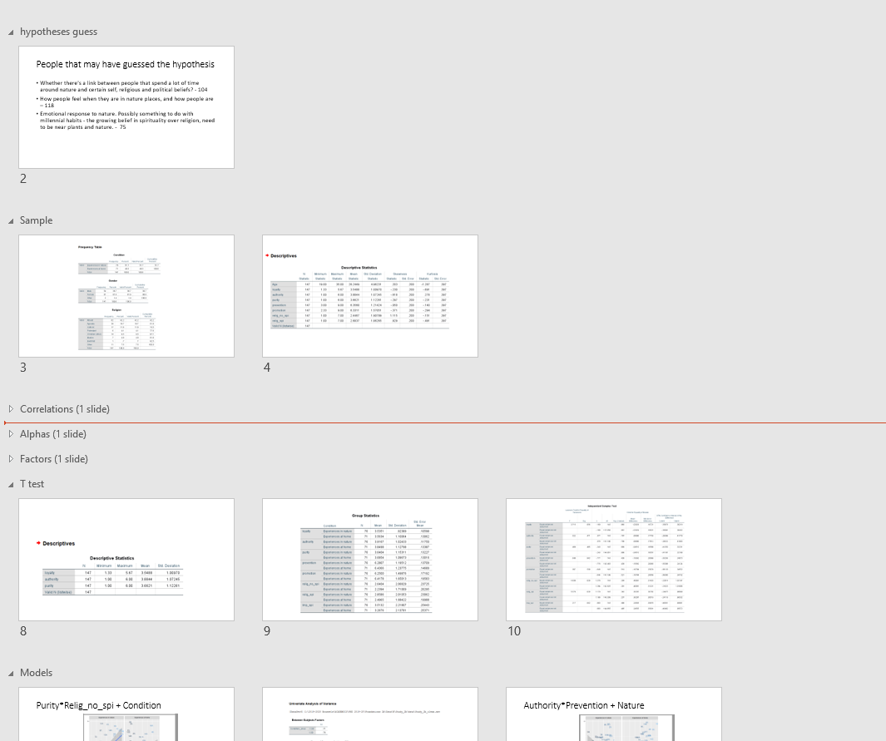
\includegraphics[width=\textwidth]{images/ppt2.png}
        \caption{Screenshot with few slides of the PowerPoint of one study.}
        \label{fig:ppt2}
    \end{figure}
\end{center}

\subsection{Bibliography: All those papers you'll never read}
\label{subsec: bibliograph}
Living in 2020 and writing the references manually should be forbidden, (unless you like some sort of academic \textsc{bdsm}). Really, develop a system of automatizing the references and bibliography. 

In my case, I use \href{https://www.mendeley.com/?interaction_required=true}{Mendeley} and the Word extension, but consider getting familiar with \href{http://www.bibtex.org/}{\hologo{BibTeX}}, and start using \ \href{https://www.latex-project.org/}{\LaTeX} or \href{https://crsh.github.io/papaja_man/}{\textsc{papaja} package} in R\footnote{The legend says that you can upload all the results and bibliography directly in the paper just by running a chunk of code.}.

For folders and sub folders in \href{https://www.mendeley.com/?interaction_required=true}{Mendeley}, you can use the organization of the literature as you previously did in the \textsc{literature} folders.\footnote{ I am not the best at managing literature, so feel free to recommend and suggest new practices. }

\subsubsection{\href{https://www.latex-project.org/}{\LaTeX} and \href{http://www.bibtex.org/}{\hologo{BibTeX}}: worthy of your time}

\href{https://www.latex-project.org/}{\LaTeX} is a wonderful tool that allows to do nice looking text like this one without worrying much about the formatting.
A good way to start is following \href{http://ptmartins.info/latex/}{this guide (Click me)} that a colleague % la niña
shared with me. Also, using \href{https://www.overleaf.com/}{Overleaf} will make the whole experience much easier. Ther you can find templates like \href{https://www.overleaf.com/latex/templates/fred-slash-uf-working-paper-template/mjnnjxzqmydm}{this one} that it will probably helping with your manuscripts. 


\href{http://www.bibtex.org/}{\hologo{BibTeX}} is a reference management software. Using \href{http://www.bibtex.org/}{\hologo{BibTeX}}, you just need to keep a horrendous miscellaneous \emph{.bib} file with all your references since you started the first year of bachelor until your current moment. Then, with a bit of knowledge about, and \href{https://www.latex-project.org/}{\LaTeX}, you can easily cite whatever you want that it is in that file. 


\subsection{Shortcuts: Increasing your lifespan second by second}
\label{subsec: shortcut}
As David Cain in its blog \href{http://www.raptitude.com/}{Raptitude} recommends: 

\begin{quote}
    \begin{center}
        \href{https://www.raptitude.com/2015/02/67-short-pieces-of-advice-you-didnt-ask-for/}{Learn keyboard shortcuts. If you don’t know what \textsc{CTRL + Z} does, your life is definitely harder than it has to be. }
    \end{center}
\end{quote}

Lean shortcuts. Seriously. It will save tons of tons of time in your life. Learn shortcuts of your working environment (Windows or Mac) \footnote{I am using Windows. If you like Steve Jobs, sorry, he is dead. } and the different software you use daily (Windows, Word, R, Google, …). Google is your friend. So, go ahead and type “Windows/Mac/R/\textsc{spss}/Word/PowerPoint shortcuts” and print some cheat sheet\footnote{I am a pro-environmental person, but printing cheat sheets is a justifiable excuse}.

Also, it is fundamental to understand what a path is in order to move around your folders. A clear case is the situation of downloading and saving a file in its proper folder (not in the horrendous \href{https://en.wikipedia.org/wiki/Hieronymus_Bosch}{Bosch’s} hell of the \textsc{download} folder\footnote{Check also \href{https://en.wikipedia.org/wiki/Pieter_Bruegel_the_Elder}{Bruegel's} paintings to increase by one the number of cultural jokes you can add in random upcoming conversations.}).

Here’s an example:

Let’s imagine you don’t find anything interesting in Facebook and decide to work for a bit. You find a PDF on the Internet that you want to download. As a proper researcher that you are, it is likely that the paper is already inside your office, in one of those unopened journals you forget why you subscribe, but you keep on receiving four times a year. Obviously, you don’t go to SciHub\footnote{What is SciHub? Never heard of it...} because it is illegal, and proper researchers pay 20\$ for a paper that they will only use for skimming through the abstract. Somehow, the PDF file is open in your web browser. So, what can you do? 

\begin{itemize}
    \item You can \textbf{Atl + Tab} %\barleftarrowrightarrowbar no he conseguido añadir el unicode ↹ 
    and move to the windows file explorer. (If it is not open, Win + E will do the magic).
    \item Your wonderful system of organization and the use of the \textbf{touch pad} (more below) will bring you to the desired folder in few seconds. (Also, \textbf{right click in the File Explorer} icon will remind you the Recently used folders. It should be there, or you have been in Facebook for too long.)
    \item There, you can create a new folder with \textbf{Crtl + Shift + N}. 
    \item Then, name it ``\textbf{\textsc{yyyy} Author, Author - Key words}'' and press \textbf{Enter}. 
    \item Inside the folder, press \textbf{Alt + D} to select the path, and \textbf{Ctrl + C}, to Copy it. (\textbf{Ctrl + A} for selecting All if you move something.)
    \item Then \textbf{Atl + Tab} % Añadir el unicode ↹ 
    to move again to Google Chrome\footnote{You may be a paranoid and use DuckDuckGo. In that case, you probably know about shortcuts already.}.
    \item \textbf{Ctrl + S} to open the download window (In options you set up that they always ask you where you want to save it. Remember Bosch and Bruegel’s \textsc{download} folder.)
    \item \textbf{Alt + D} to select the path, and \textbf{Ctrl + V} to paste it. \textbf{Enter} to go to the folder. 
    \item \textbf{Enter} to save it. 
\end{itemize}

If you repeat this operation few times, you can automatize the movements. Get familiar with paths and shortcuts. You will be able to perform this common operation of creating a new folder and download a file in that specific place in few seconds, without using the mouse. This will save tons of time on the long term and it will make your grandmother think you are a computer wizard. No worries, if you just learnt this, you are not.

Also, \textbf{learn to use the touchpad} of your laptop and personalize different gestures. In my case, I usually have (at least) two desktops\footnote{ADHD can manifest in the form of 4 desktops, 3 Google Chrome windows with 5 to 20 navigation tabs in each. For those that love math: 60 things going on in the best of the cases, and 240 when I decide it’s time to see if there are cookies left in the kitchen table.} . Using four fingers right and left, I can switch among them. The main desktop is for music and distractions (what did you expect?), and the secondary one for work. Thus, if your advisor suddenly appears in your office, you can quickly look like a productive and industrious researcher. Very important as well, three fingers up and down, regulate the music, and tapping with three fingers stop it. 

For moving around the Folder Explorer, I use the three fingers right and left to move forwards and backwards. In Google, I the three fingers are for navigate back and forth, while the Ctrl + Tab %↹ Add the unicode again 
for moving around my tons of simultaneous searches. I recently discover that Ctrl + Number, takes me to the number of the open tab in that window. Number 9 takes you to the last, so between the 8$^{\textnormal{th}}$ tab and the last, I have a void of shortcuts. \textbf{Conclusion}: personalize your touchpad and make some use out of it. 

\textbf{Moral}: Get familiar with shortcuts, print cheat sheets, learn them little by little, and use them as often as possible. The more you can automatize, the more cognitive effort you can invest in more creative, and interesting tasks\footnote{Or coming back to your dopamine hits from scrolling the Facebook feed.}. Don’t waste your time repeating yourself or struggling going up and down the folders of your laptop, trying to remember where you should save your files. 

\section{Statistics: Not that difficult}
\label{sec: Statis}
\subsection{Where to start}
\label{subsec: start}
If you don’t know statistics, the best is to enroll in a course of the faculty. In case you did learn statistics and want to refresh concepts, Andy Field’s books are good sources. Go to the library and get them.
\begin{itemize}
    \item \emph{An adventure in Statistics} \citep{field2016adventure}, if you have time and want to enjoy the process of learning. 
    \item \emph{Discovering statistics using R} \citep{field2012discovering} or \emph{Discovering statistics using \textsc{spss}} \citep{field2013discovering} depending on the program. They are basically the same in the theoretical chapters (the firsts ones), which I strongly recommend reading. 
\end{itemize}

\begin{flushleft}
Other handbooks that you may want to have are\footnote{Add your favourites to the list, and we all learn from them}:
\end{flushleft}

\begin{itemize}
    \item \emph{Data Analysis: A Model Comparison Approach} \citep{judd2011data}
    \item \emph{Handbook of Research Methods in Social and Personality Psychology}\citep{reis2000handbook}
    \item \emph{Intro to R for Psychologists} \citep{nydick2013intro}

\end{itemize}


\subsection{How to learn R independently}
\label{subsec: learn R}

I have used two main books in my R journey:
\begin{itemize}
    \item \href{https://bookdown.org/ndphillips/YaRrr/}{\emph{Pirate guide for R}} \citep{phillips2017yarrr}. It is funny and easy to use.
    \item \href{https://r4ds.had.co.nz/}{\emph{R for data Science}}. I read it pretty much completely, but you may not need to.
\end{itemize}

\begin{flushleft}
A suggested order for exploring these two books is:
\end{flushleft}

\begin{enumerate}
    \item Read chapters 1, 2, and 9 of Yarrr book, download, install the program and get organized. (Chap 9 can be confusing, skim through it to get the idea, and come back later.)
    \item Read 3 to 6 of Yarrr to learn basics. 
    \item From R for data Science read from 1 to 6, skipping the third if you want. (Chap. 3 can be a bit confusing.)  
    \item Then feel free of exploring at your own. Using R4ds can be great to learn \href{https://www.tidyverse.org/} {\emph{tidyverse}}\citep{wickham2017tidyverse} and \href{https://ggplot2.tidyverse.org/}{\emph{ggplot}} \citep{wickham2007ggplot} packages directly. However, it is good to get the basics of R using Yarrr.
\end{enumerate}

\begin{flushleft}
\href{https://rstudio.com/resources/cheatsheets/}{Clicking here}, download and print the following cheat sheets. 
\end{flushleft}

\begin{itemize}
    \item Data visualization
    \item Base R
    \item Apply functions
    \item Data transformation
    \item Factors with forcats
\end{itemize}
There are more you may need on the future, but these are basics.
Also, it is important that you know \href{https://stackoverflow.com/}{Stack Overflow} . It is the place where you'll find the answers of most of your questions. 



\subsection{Best of R}
\label{subsec: Best R}
You should learn R for several reasons. 
\subsubsection{Keeping track of cleaning data process}
\label{subsec: track cleaning}
I really encourage learning R for writing and keeping a record of your modifications. Specially during the first steps, where you are very excited about getting your freshly baked data. You move around changing names, computing variables, making calculations… But before getting disappointed because your hypotheses weren’t confirmed, you may want to register what changes you are doing for reporting later. With R, there is no other way than writing and saving the code, which is a form of registration. Therefore, use R for cleaning the data

Having an understandable R script, you can go home happily knowing that the day you will write your dissertation in the loneliness of your office, you will not have a panic attack trying to remember what you change in your data set three years ago.\footnote{I am a non-Ph.D. and I haven’t written any dissertation, so maybe that anxiety joke it is all a lie and finishing up your Ph.D. is like partying at Tomorrowland. Who knows?} 

With the code, you register the cleaning process, step by step. How you imported the original dataset, the names you changed, the calculations to create new variables, the operations you made to get your results, and how you exported the dataset for sharing. This is fundamental. Keep it on mind. You will save lots of suffering trying to remember that thing you did once upon a time, in a grey Belgian morning of a forgotten month of October.

\subsubsection{Iterations, and exploring your data}
\label{subsubsec: iterations}
R is not only for registering and saving your process. R is a computing language, and if you were surprised with the trick of the shortcuts, now your grandmother will start thinking that you actually know how to use a computer.

Computing machines are for avoiding humans repeating themselves. Google “Don’t Repeat Yourself”. Thus, if you ever found yourself in SPSS, making graph after graph, changing variables, adding or deleting outliers, or stuff like that, you have here an opportunity of changing your destiny.

I simply refer to the books of before (\emph{Yarrr} and \emph{R for data science}) for more information.

Apart from the cleaning process, I find R especially useful for exploring your data\footnote{  I will not get into debates about good research practices, data dredging (p-hacking), etc. I assume that you will explore your data for designing more nuanced studies and hypotheses in the future.}.  The power of computing here is that you can make statistical models, regressions, and graphs for pretty much every combination of variables. Make a vector of independent variables, another of independent variables, another of moderator. Then, ask the computer to combine all of them. If you have written a proper code, you can reuse for your next studies.

\paragraph{Valuable sources of information}
\label{parag: sources}
\begin{itemize}
    \item \href{https://aosmith.rbind.io/2018/08/20/automating-exploratory-plots/}{\textbf{Automating exploratory plots with ggplot2 and purrr}}:A bit advanced, but this code is gold 
    \item \href{https://github.com/seanchrismurphy/A-Psychologists-Guide-to-R}{\textbf{A psychologists guide to R}}: A former post-doc share it with me. I never got very familiar with GitHub, so I am not sure how to use it, but the name is promising. 
    \item To be added by you \smiley{}
\end{itemize}


\subsubsection{Sharing and reusing code}
\label{subsubsec: Reuse}
One of the best things of R is that you can use the same code for different studies, and share it around the internet, so other people and colleagues can benefit from your work. I have written some code myself that I have reused in several studies. In my case, it is an experimental between-subjects design with an experimental variable and a control variable. Email me if you are interested on taking a look at it. (I may upload it somewhere in the near future, but the near future of an ADHDer can be extended \textit{ad infinitum}.
\subsection{SPSS. What for?}
\label{subsec: SPSS}
Under the pressure of my advisor, I learned how to use \textsc{spss}. It is not difficult and it can help complementing and double checking that you are not messing up with R. Also, I discover that it is quite handy for doing basic analysis. Mainly, I didn't have enough time to delve in R to get ways to perform the operations automatically. Therefore, nowadays, I use \textsc{spps} for: 
\begin{itemize}
    \item Descriptive statistics: frequencies, mean, standard deviations…
    \item Correlations (I found a code for getting the same table with stars output in R, but life, you know…)
    \item Alphas
    \item Factor analysis
    \item T-test
\end{itemize}
\begin{flushleft}
However, I would never use SPSS for doing:
\end{flushleft}
\begin{itemize}
    \item Graphs: With an iteration code, I can make 90 graphs in 1 minute in R.
    \item Linear models and regressions. R saves you the annoyance of creating new variables just for running a model.
\end{itemize}
\begin{flushleft}
I didn't get to explore and understand mediations and moderations. So, you will tell me.
\end{flushleft}


\subsection{G Power}
\label{subsec: G Power}
You can check in a statistic handbook what and how to calculate the power of your experimental research. You can download G*Power and its manual \href{http://www.psychologie.hhu.de/arbeitsgruppen/allgemeine-psychologie-und-arbeitspsychologie/gpower.html}{clicking here}  

\section{UCLouvain specifics}
\label{sec: UCLouvain}
In the best of the cases, your secretary has sent you an updated version of the \textsc{ipsy vade-mecum}. There you can find a lot of useful information. However, I decided to make my own step-by-step guides because I was receiving the same questions from my colleagues. \footnote{Most of this section has hyperlinks, so read moving your mouse around the text, for not skipping any of them.}

\subsection{How to get the ethical approval?}
\label{subsec: ethic}
How to get the approval from the ethics committee? (November, 2018)
\begin{enumerate}
    \item Go to the main \href{https://uclouvain.be/fr/instituts-recherche/ipsy}{\textsc{ipsy}} page. The sooner you get familiar with the page, the better.
    \item On the upper part, click on the menu ``A propos''. Then, ``Commission d’Éthique''.
    \item Once \href{https://uclouvain.be/fr/instituts-recherche/ipsy/commission-d-ethique.html}{here} you are welcome to read the information. 
    \item At the left, in \href{https://uclouvain.be/fr/instituts-recherche/ipsy/composition-calendrier-criteres-d-evaluation.html}{``Presentation < Composition, calendrier, critères d’evaluation''} you can find the next meeting of the commission, and the limit for new demands. Those two days are important. Keep them handy.
    \item In ``Presentation <  Outils et références''. You can click on `` Demande d’approbation'' Feel free to read the text, and look around the site.
    \item Read the information on \href{https://uclouvain.be/fr/instituts-recherche/ipsy/demande-d-approbation-d-un-programme-de-recherche.html}{``Demande d’approbation''}.
    Some links don’t work; e.g. \textsc{demande a la commission d’ethique d’ipsy}.
    \item Click in ``volets \textsc{a-bcd}''. Hopefully you have Microsoft Office, because the file is not so friendly with other word processors. 
    \item Fill up the file with your information and the information of your project.
    \item Take a look at the ``Outils et références'' page to check that you don’t need to fill others docs; e.g. minors, or filming)
    \item Take a look at ``Consentement'' for redacting your own texts. 
    \item Take a look at ``Recommendations''. There is information about
    \begin{itemize}
        \item ``General ethics principles'', 
        \item ``Internet surveys for research''
        \item ``Retribution'' to participants
        \item Also, if you want participants, you can click on ``Charte des experimentateurs'', and contact \href{mailto:martin.edwards@uclouvain.be}{Martin Edwards}
    \end{itemize}
    \item After completing the files, send them to \href{mailto:demande-ethique-ipsy@uclouvain.be}{demande-ethique-ipsy@uclouvain.be}  
    \item Keep on mind that the ``Mise à jour'' is an update of a previous project. In case you make modifications, or change anything, the correct procedure is to inform the ethical committee about it and send an update it about it. 
\end{enumerate}


\subsection{How to activate your Qualtrics account?}
\label{subsec: Qualtrics}
How to activate a Qualtrics account? (November, 2018)
\begin{enumerate}
    \item Email \href{mailto:Nadine.fraselle@uclouvain.be}{Nadie Fraselle} \textsc{gestionnaire de recherche} and inform her about your status, name and surname, and name of promotor. 
    \item She will email back a document that you have to read, sign, and re-send.
    \item Later on (one or two work days), \href{mailto:Dominique-Robert.Hougardy@uclouvain.be}{Dominique-Robert Hougardy} \textsc{(support technique, multimédia)} will send you a presentation with the instructions to access the platform and create you survey. 
\end{enumerate}
Feel free of uploading a link to the PowerPoint with the instructions sent by Dominique to the guide.


\subsection{How to book a room or a lab}
\label{subsec: book}
For booking a room or a lab, do the following. 
\begin{enumerate}
    \item Login in \href{https://sites.uclouvain.be/reservation-psp/login.php}{here} 
    \item In the left menu select ``Labos Niveau – 4'' or other. 
    \item Click on the + sign and fill the form. 
\end{enumerate}
\textbf{Pro-tip}: If you want to book more than one day at once (e.g. you are running an experiment for several weeks), change the ``heures'', by ``jours'' or ``semaines''. It took me a bit of realizing it, and I was booking single days repeatedly because, you know, life.

\subsection{Using Martin's Edwards pool of participants}
\label{subsec: Martin}
\textsc{how to find students for your research using martin edwards pool of participants?}
\begin{enumerate}
    \item Send an email to \href{martin.edwards@uclouvain.be}{ Martin Edwards}
    \item He will send you a PDF file with the instructions and information. You can also find the file \href{https://uclouvain-my.sharepoint.com/:f:/g/personal/carlos_alcala_uclouvain_be/EmwYTCf0VTBKm5ce0Nf_TRYB_VKXQbs4sqOtW1MwRyzAyw?e=5RpmwF}{here}
    \item Read the instructions and write the files needed and send him. I leave a samples linked.
    
    \href{https://uclouvain-my.sharepoint.com/:b:/g/personal/carlos_alcala_uclouvain_be/EaWQ80YJY8tLqHQrZkXlEn4B6N1usGtCU9Ab-w-70-gI8Q?e=3hnbB1}{Signed experimentation instructions}
    
    \href{https://uclouvain-my.sharepoint.com/:w:/g/personal/carlos_alcala_uclouvain_be/EedncL2exzBElNTLh96RxE0B8yf0Zs67iWZ7M8VqDEIXmw?e=sFNc5Z}{Consentement eclaire}
    
    \href{https://uclouvain-my.sharepoint.com/:w:/g/personal/carlos_alcala_uclouvain_be/Eek6vCacUeNPnDZGVa4Df6YBCRkqaAqJ8SqiSNHXUixhBQ?e=KGjP9L}{Information about the experiment}
    
    \href{
https://uclouvain-my.sharepoint.com/:w:/g/personal/carlos_alcala_uclouvain_be/EaKt779vejZMq4uhbPjtS1ABOG7xuaTgr2IpeSuw-y8how?e=wqOlaO
}{Information to the participants}

    \item Once all the information has been sent to Martin Edwards, he will give you access to the platform, where you can open a new folder and then upload the files with the information. 
    \item 	You are supposed to book the rooms for the experiment \href{https://sites.uclouvain.be/reservation-psp/login.php}{here} 
    \item If you get lost, you can send him and email and ask.
\end{enumerate}

\subsection{How to download your data from Qualtrics?}
How to download your data from Qualtrics (February, 2020)

It is recommendable to read about different types of tables and formats that save data. You can find this type of information in R for data science by Hadley Wickham. Check section about R. 

Click on your study $\rightarrow$ Data \& Analysis $\rightarrow$ Export \& Import $\rightarrow$ Export Data $\rightarrow$ \textsc{spss} $\rightarrow$ more options $\rightarrow$ Export viewing order for randomized surveys (If you want to get more information for later analysis.)

You can also download an Excel or \textsc{cvs} file if you are up to. But downloading the \textsc{spss} file and then using the package ``Haven'' to work in R should be good. 

\subsection{How to get refunded?}
\label{subsec: refund}
If you carry out an online survey, you pay the inscription of a conference, or book a hotel room, you probably want your money back. 
Save all the tickets and place the files in a place that is easy to retrieve in the future. The system got digitized and automatized. \footnote{  It is 5.30 a.m., I have been writing since 2.30, and I am tired. Since, this is the section of money, western individualistic societies are quite concerned about material wealth, and I already got refunded, let’s see if the reader is up to updating the guide with some basic instructions. \smiley{}}

\subsection{How to get your commuting card?}
\label{subsec: commuting}
Waiting for your collaboration. 
\subsection{How to enroll in Moodle courses?}
\label{subsec: Moodle}
Waiting for your collaboration.
\subsection{How to enroll in PSYCEDUC courses?}
\label{subsec: PSYCEDUC}
Waiting for your collaboration.


\section{General life advice: I am not your grandma but...}
\label{sec: life advice}
Since you have gotten this far, I guess you assume I store some valuable information in my mind. In a similar way as David Cain, writer of \textit{Raptitude}, here is a quick list of my habits and practices for a good life.\footnote{If you want to know more, I have a blog where I post different types of things from type to type. You may find something useful there as well. \href{www.carlitofluitoideas.com}{Carlito Fluito Website}.  One of my current life goals is to become a full-time artist, including writing, and posting regularly. Good vibes and support is always welcomed.}  They evolve from more to less work related. Feel free to stop reading whenever you want. \footnote{ This is the classical ``I am not a doctor'' message. Use your common sense, take all this practices as a personal exploration sort of game, and never put your well-being under extreme situations or circumstances. If you are like me, you probably don’t care and you’ll end up doing what you want, but at least, I will sleep better knowing that I wrote this small warning.}

\subsection{Be social}
\label{subsec: Social}
I decided to place this one the first because one of the main reasons I am leaving this country and this job is the lack of love. Love manifested as positive and meaningful social relationships. Doing a Ph.D. is an already quite isolating job, and in a country like Belgium, or a city like Louvain-La-Neuve, you may find difficulties to find people you connect with. Social isolation and loneliness is an epidemic in individualistic societies. The institutionalized social services take care of those in risk, but the lack of an organic and natural social network can be hugely damaging for individuals and society as a whole. I don’t blame individuals; I think the whole problem is structural. Nevertheless, this is probably not the text to write about it. The thing is, you have a opportunities of socializing every day. Sometimes you will not feel like doing it, but try anyways. 

\subsubsection{Make questions to other people}
\label{subsubsec: ask others}
I hope this guide contains some answers to your potential questions. However, feel free of getting to know about your colleagues. Don’t only ask job-related things, you can slightly move to more personal topics. As an \textsc{adhd} Spaniard, some people find me too straight-forward or weird. Don’t worry much about what other people think, I probably said and did something more stupid than what you may say or do. 

\subsubsection{Have coffees, lunch or dinner with your advisor and colleagues}
\label{subsubsec: coffees}
Try to make your breaks as social as possible. If there are people having lunch in the kitchen, pop up. If you have extra-coffee, or extra-tea, offer them a cup. Be proactive and suggest going for lunch or dinner outside the building, and if possible, outside the city. Don’t underestimate the power of social ties. 

\subsection{Workflow}
\label{subsec: workflow}
Working is one of the things more difficult to escape in this civilization. I am working on it. For the moment, at some point you will have to work. Thus, try to make your life easy, and use the resources of the university. 
\subsubsection{Drink lots of water}
\label{subsubsec: water}
Classic one, but extremely important. One of the things I do when I arrive to my office is filling three bottles of water. Then I struggle opening the doors in the way back, but I like the game as well. Other people say that it is better to have just a glass to force yourself to take breaks often and move your body. However, my chronic procrastination tendencies have shown me that if I start doing something, it is better not to get distracted. 
\subsubsection{Chronotypes}
\label{subsubsec: Chronotypes}
Learn about your brain. This civilization is designed by and for average boring sapiens. I am a weird one. Daniel Pink wrote When: The scientific secrets of perfect timing. You can look like a smart psychologist if you mention some of the research presented on the book on your social gatherings. However, the real utility may lay in understanding why I am unable to do anything in the morning, why Wednesdays are for me a waste of time, and when is best for me to exercise (all the time, actually). Thus, there will be moments and days for writing, others for reading, and others for walking around the lake. Learn about which one is which for you, and you may save hours of struggling in front of your laptop.
\paragraph{Night owls}
\label{parag: Night}
If you are as lucky as me, you function better one evenings and night. A lifestyle that is designed for people that wake up refreshed at 7am, can be a torture for those that go to sleep at 4am, fully satisfied for working uninterruptedly for 5 hours straight. Professors at psychology faculties should be aware of these realities. Sometimes, they may not. Anyways, try to negotiate and argue your work schedule. You can get a pass card to enter and leaving the building after 20pm and find people that socialize in the mornings. It can take some time, but it is doable. If not, escape the system.
\subsubsection{Binaural Pomodoro}
\label{subsubsec: Pomodoro}
This one is original\footnote{Avoid plagiarism and reference the source.}. Many people are familiar with the Pomodoro technique (work 25 min, rest 5). In my case, since I have difficulties to start working, I usually cheat my brain making it belief that I will take the break when I won’t. However, I like to keep track of time and know how much time I have spent working and how productive I have been.

Since silence can be a torture and music too distracting, I have found a middle point on binaural beats. You can google it and find out the not-scientifically proven wonders of these sounds. In my case, I like \href{https://www.youtube.com/channel/UC6RzukLXWGBx6dOGqzaeK5w}{``Jody Hatton's Videos''} in YouTube. I play the 25 Minute POWER NAP, and I use it as a Pomodoro timer. In a productive way, I can play it on repeat two or three times, getting a full hour and a half of productive and focused work. 

There is also a track called “90 minutes of focused studying”, that you may like. The guy has videos explaining how to use the beats, and its potential benefits, depending on the wave and sounds. Explore his channel. 

\subsubsection{Deep work}
\label{subsubsec: Deep work}
This is the Promised Land that I have seen in distant mirages when I am in the desert of continuous social media distractions. You can check \href{https://www.calnewport.com/books/deep-work/}{Cal Newport’s book} for more information. In my case, I work best at nights without distraction and with my phone purposely left at home. I have tried many systems for blocking websites and apps, but I have ended up finding a way around all of them. Anyway, start with the basics, do yourself a favor, and set Airplane or Silent mode in your phone when you have to work. 
\subsubsection{Set personal deadlines before the Deadline}
\label{subsubsec: deadlines}
I am a professional procrastinator, and my brain lacks the necessary sensitivity to dopamine and norepinephrine to feel any type of fear or anxiety when deadlines are approaching. I have been able to prepare presentations of conferences in the hotel room. I have spent whole nights self-punishing my ridiculous distractions because I just had 2 hours left, and I the thing wasn't finish. So, believe me on this. Set your own personal deadlines at least 3 or 4 days in advance of the actual deadline. Shit happens, and shit will happen. This universe has a potential of infinite last-minute unpredictable situations that can screw you up. Be serious with yourself and try to hit your own deadline. In the worst of the cases, you still will have 72 hours to go. 
\subsubsection{Get an extra monitor}
\label{subsubsec: monitor}
If you have a small laptop and you are using only your screen, you are making your life difficult. Ask for an extra monitor to the IT responsible. You will perform many tasks way more smoothly. Browsing the internet and saving literature, working on several files simultaneously, fighting with your code and deciphering the solution offered in Stack Overflow. It will save the functional life of your eyes, and column.
\subsubsection{Get a mouse if you need to}
\label{subsubsec: mouse}
For an average research job, you may not need one. If you learn a few shortcuts and have a nice touchpad, it should be fine. However, if you feel that you need one, ask the IT responsible.
\subsection{Take breaks}
\label{subsec: breaks}
Unless you squeeze the precarious moments of focus as much as I do, your body and mind will thank you some rest.  As a general rule, do the opposite of what you have been doing. If your work consists on being seated on a chair, alone, in a closed space, staring at a screen shooting photos straight to your pineal gland; you may need some movement, socializing, fresh air in an open space, and some sunlight. 
\subsubsection{Interacting with other living creatures}
\label{subsubsec: interact}
As I said before, social relationships are much needed. Placing a living being in your surroundings, like plants in your office, although very beneficial, can be a bit boring. Thus, try to find other living forms with whom you can interact and communicate with. People will shoot a combination of adrenaline, dopamine, serotonin, and maybe oxytocin in your nervous system that will wake you up, motivate you, make you feel good and happy, and maybe make you prone of developing some long lasting bonds. The world is full of free walking pharmacies. Take advantage of it.

\subsubsection{Exercise, stretch, and move}
\label{subsubsec: Exercise}
Similarly, there is tons of books, papers, and information about how our body, as animal’s body, is designed to get its daily dose of movement. In a desk job, it is likely our lives are movement deprived. I always lack the constancy and will-power needed to do 30 squats, or 15 push ups every 25 minutes. However, I know people that actually do it. Give it a try, your body and brain will thank it. 
\subsubsection{Meditate}
\label{subsubsec: Meditate}
There are tons of literature about the somehow scientifically proven benefits of meditate. My advice is to do a one single case qualitative introspective experiment with yourself and give it a try. \href{https://en.wikipedia.org/wiki/Jon_Kabat-Zinn}{Kabat-Zinn}, \href{https://www.raptitude.com/}{David Cain}, and even Carlito Fluito\footnote{Yes, self-promotion. \href{https://www.carlitofluitoideas.com/meditation-app/}{Click here}.} are good starting points. Sitting outside, taking some fresh air, and focusing for 20 minutes on your breath can reboot your brain, and make you successfully tackle that task you have been struggling for the last 3 hours. 
\subsubsection{Power Naps}
\label{subsubsec: Power Naps}
No one has ever done it. Me neither. However, if you want to be the first person that tries it, you can lock your office from inside, set an alarm or putting a binaural beat sounds, and lie flat on the floor of your office. It is worthwhile, since you are probably sleep deprived, and your brain is not working properly. You can refine the technique as much as you feel like. Maybe, you can put on the hood of your feather coat, lay down a chair, place some journals below the backrest to get the desired height for a perfect pillow, lie on your back, and put your hand in the pockets. Never tried, though.

\subsection{Life habits}
\label{subsubsec: Life}
In this last section I am going to proselytize a bit. I have been described as ``singular'', ``uncommon'', and ``atypical'' by my advisor.\footnote{I even have a \href{https://www.youtube.com/watch?v=4lvSzHfc8FU}{documentary in YouTube about my life in Brussels. Click here.}. } However, I still stand for continuing with the researcher project of myself (my neurological, physiological, psychological, body, and spiritual functioning). Whether your life is sweet or shit, you will have to share that experience with yourself. Therefore, investing some time in figuring out who the hell are you travelling with in this life journey can be of immeasurable utility. Make your personal self-knowledge a life habit. \footnote{I plan to post individual entries in my blog about some of these topics. Thus, take a look if you are specially interested in any of these and want some detailed information. \href{www.carlitofluitoideas.com.}{Carlito Fluito ideas}. If you don’t find them written yet, I am still postponing the task. It happens. Thanks for your patience.}
\subsubsection{Brain caring}
\label{subsubsec: Brain}
I am not a neurotypical person. Causing the mockery of my unsurprised social network, I have figured out about my ADHD brain at 27. Thus, you may find excessive some of the following advices. However, considering the pseudo-ADHD civilization of constant interruptions and instant messaging that we are building, you may benefit from those of us that have a clearer phenotype. 
\paragraph{Focus on growth: Update and improve attitude}
This can be a bit too much self-help, self-improvement advice but it certainly works. Try to keep yourself on the line between satisfaction of what you have and dissatisfaction of what you are missing. This way, you will remain growing and growing. Challenge your beliefs from time to time, keep on learning new things, and try different strategies and techniques to see if you can improve different aspects of your life. Nevertheless, don’t go too individualistic, keep your social connections tight and supportive. Growing together feels better than growing alone.
\paragraph{Develop habits and routines}
It can be difficult when you lack social support and people to do your routines with. But if you force yourself long enough, you may end up being addicted to meditate, exercise, and having cold showers first thing in the morning. Thus, the day you skip your routine, your being will feel it and give you some gentle reminders throughout the day. Find a system for tracking them, so you can fight self-delusion with the power of a Yes or No sign throughout the month. 
\paragraph{Become minimalist}
As ADHD, I usually struggle a lot with too many items in my working memory. One of the best ways I have found to move more smoothly through life is reducing as much as possible the unnecessary objects in my life. The book Essentialism can help you become minimalist further than material possession. In any case, I advise you to start with the kitchen. If you are living alone, or a shared flat, having one glass, one plate, one set of cutleries, one pan, and one casserole, will significantly reduce the amount of time that you spend doing dishes. Extra aspects are that you will automatically become more environmentally friendly, your finances may be benefited, and you’ll save time for meaningful things, and you’ll grow more independent of material wealth, facilitating your escape from the system. 
\paragraph{Phone fasting}
My altered dopaminergic system has a love and hate relationship with the smartphone. It is incredibly useful to read books, listen to music, or writing down the to-do list for the day while I commute. However, it is deeply disturbing for my attention check repeatedly Facebook, Instagram, and Whats App to be updated about my last social interactions. Therefore, I developed a routine of not checking social media before 12 am. Whatever the message I had received, the sender could wait some hours for my answer. When people seriously want something, they will call or SMS you.  Give it a try. In my case, the effects were clear and powerful. I was able to keep my dopamine levels under control, sustain my attention for longer and struggle less with distractions. 
\paragraph{Sleep and disconnect}
I never had problem sleeping, but many people do. Thus, if that is your situation, you probably know how important, regenerative and healing sleeping is for your functioning. There is ton of information about it, on the internet. I am not an expert, but for sure that disconnect from devices, drinking an herbal infusion, and meditate will help. 

\subsubsection{Body caring}
\label{subsubsec: Body}

The body is that thing that move our consciousness around. Although, I could go further and say that the body is an extension of our consciousness. Besides, it is the way we interact with the physical realm of this reality. Therefore, you have substantial reasons to take care of it. In my personal case, the whole thing gets even more meaningful since I want to develop a career as dancer and performer. Thus, my main tool is my body, and I want to make it function as much as possible. 
\paragraph{Shower with cold water}
It is a pain on the ass. It is easier to make it in the summer, and again, it seems that people that feel lonelier spends longer time under hot water than those that feel socially connected. You can research a bit on the internet, check the Wim Hoff Method, and start progressively. You will realize that cold exposure will help you remain healthy, avoid catching colds, feel warmer during the day, improve your skin in case of dermatitis, give you a boost of energy, and cool down your emotions. Try to develop the habit, it is really worthwhile.  
\paragraph{Exercise, stretch, move, dance}
You know this already. The body is designed by evolution to move every day. We are animals that were raised on the wilderness. These days, we are living in cages we call rooms and offices. However, we need to move, the whole system works better when you do. A little is better than nothing. So, don’t do like me, and think that for only moving 5 minutes you are not making any change. Taking the stairs is more movement compared with the elevator. Start easy, go progressive, build the habit solidly, and keep on challenging yourself. 
\paragraph{Squat shitting}
In the developing parts of the world, this is the rule. It is us, WEIRD’s that want to do everything against our nature. The body is designed to evacuate in a squat position. It is what it is. I do it since 2016. It is automatic, it doesn't cause me any extra effort, and when I sit on the toilet, I feel weird. It is more difficult. I have a video on YouTube explaining the perfect technique. Go check it out. Your vowels will thank you the change. 
\paragraph{Sleep on the floor/hard surface}
This is the most extreme. I have been trying for some time and the body ends up getting use to it. In my room, I have carpet floor. Thus, you may want to start with a futon, a tatami, or lying over a duvet. Sometimes I sleep on the bed as well. However, I have noticed that with the right height for the pillow, I end up feeling better in the morning. I recover much faster, and it also allows me to sleep pretty much wherever when I am travelling. Give it a chance.

\textbf{Pro tip}: Usually, for males, the shoulder size is bigger than for females. And for females, the waist is wider. Thus, play a bit with the pillows if you sleep on the side. If you are a man, you may need more pillows to avoid your head hanging, and if you are a woman, you may need some pillow at the belly level to avoid the waist bones sticking out.

\subsubsection{Dietary habits}
\label{subsubsec: Dietary}
I am a bit extreme with the following ones. I believe that we are what we eat. What you put in your body becomes your cells. Also, I think that diet is one of the unavoidable environmental impact that we all humans have. Therefore, I try to be conscious about my decisions, where do the food I consume come from, what is the impact, and how it is going to affect my body. However, when lack of social relationships hits, then I fall into bad habits like sugar, because, you know, we all need to get serotonin somewhere.
\paragraph{Go vegan, raw vegan or frugivore}
If you like being alive, animals like it too. It seems that the pulse of survival and freedom in inherent to all lives form. In case you don’t empathize enough to stop drinking milk, you can start with stopping eating meat from mammals. Just take it step by step and making all the way down the animal kingdom. Going vegan is just showing care and respect for other beings. It is that simple. Take it is as an improvement path. It is not extremist or radical, quite the opposite, systematic torturing and slaughtering of enslaved species seems more extreme and radical from my point of view. It is not about moral hierarchies, it is about doing what you feel and know as right. Simple. 

Extra aspects of going vegan, it is more environmentally friendly, shopping will be easier and cheaper, your body functioning will improve. If you go a step further and become raw vegan, you can save tons of time on cooking. If you go a step further and become frugivore (with some nuts and green leaves), you can change the whole functioning of your physiology and body, save tons of time and money shopping, and reduce your environmental impact at the lowest. Read 80/10/10 diet to get an idea of the ideal to reach. After that book, at least, you will go vegetarian.

\paragraph{Avoid processed foods and refined sugars}
If you go vegan or beyond, this is extremely obvious. However, if you know me, you know that my impulsivity can manifest in refined sugar and patisserie cravings (which may not be even be vegetarian). Be gentle and avoid self-punishment, but always strive towards a better version of yourself. Treat yourself properly and don’t contaminate your body. If you experience cravings, those are probably emotional needs that go unfulfilled. Invest in your social network. 
\paragraph{Food fasting}
You may have heard about intermittent fasting. Give it a chance. In my case, it helps me to keep my dopamine levels balanced, especially in the morning. Read a bit and try it out. Start with 12 hours, postponing breakfast; and aim to a sustained 16 or 18 hours (or beyond if you feel like). Fasting is the most scientifically proven strategy to lengthen your life. If you like your life, you may want to experience some hunger from time to time.
\paragraph{Drop caffeine}
Substitute it with water, tea, or herbal infusions. You can still use it from time to time as a mild psychedelic altering consciousness substance but try to keep it under control. If you are taking more than two coffees per day, you probably need to chill down. 
\paragraph{Try teeth cleaning twig}
As with (raw) vegan and frugivore diet, seems that hunter-gathered uncivilized life-style is the one our bodies and brains were designed for. Thus, play with primate cleaning practices as cleaning your teeth with parts of trees. You will help the environment by dropping plastic toothbrushes and dentifrice packages. 
\paragraph{Drop plastic and extra packaging}
In accordance with the minimalist and pro-environmental advice. It is likely that you don’t need much of the plastic you consume, and if you accumulate it out of guilt, you may end up with half house full of plastic bags, small packages, and so on. I have been there. I know it is difficult but just try to be conscious about it. The planet is already quite full of plastic. Also, you can start a citizenship movement to make a campaign for pressuring new policies. That would help for sure. 

\subsubsection{Soul caring}
\label{subsubsec: Soul}
I am aiming to become a spiritual psychologist, whatever that means and no matter if that exists or not. Curiously, it is somehow reiterative, since the whole discipline is called psychology (psycho – soul, logos – knowledge). Thus, a soul or spiritual psychologist is someone that specializes on the study of the soul’s soul. Anyway, I don’t think all psycho-socio-cultural, physio-bio-neurological processes concerning human spirituality (whatever that means) are not very well researched. There is a big debate about what is and what is not spiritual, but this is not the place for these discussions. I got specialized in positive psychology, psychology of religion, moral psychology, and environmental psychology, so let’s imagine that a inputs from these disciplines can be easily related with human spirituality. 
\paragraph{Explore your consciousness}
Meditation is the key tool for observing the workings and functioning of your own mind. From the most basic exercise of attention to the breathing, and observing your body, to those more esoteric one concerning energies, and visualizations, feel free of developing alternative mind states. Scientific or not, nobody is being hurt because you try. If it works for you, shouldn't you use it because there is no scientific evidence? When we behave as individuals we don’t have to be academics, we can also enjoy our beliefs without knowing the working mechanism. 

There is also a wide list of other practices you can do to explore your consciousness. Some of them are through sounds, like mantras, ohms and gong baths. Some are through your body, like ecstatic dance or physical stimulation. Some are through the environment, by feelings of awe in the nature. Some are with other people, by making love and having orgasms. Some are with external substances, like trying psychedelics. Don’t think that your daily state of consciousness, the way you often perceive reality is the only way that exists, or it is the right, proper way. After all, in our civilization it is common to drink coffee in the morning to feel more alert, alcohol in the evening to socialize, and watching a film to relax. So, why shouldn't you go a step forward sand find out what is the best practice for your type of brain to set up your consciousness in the desired state for a given situation? My little warning is that you explore your consciousness consciously. You probably don’t want to be as crazier than the craziest, but just crazier than the sanest. 
\paragraph{Prioritize love}
Use love as a guiding principle in your life. Love the things you do and love the people you are with. Try not to buy the lies of the economic system that suggest that sacrificing social relationship to get individual goals will bring you happiness and fulfillment. Wellbeing’s key component is other people. Invest in your social relationships and dare to go further. Aim to develop meaningful and long-lasting bonds with people that understand and supports you. Isolation is dreadful and feeling lonely can be the beginning of a downward spiral where you may lose the motivation for doing anything else. Use your feelings as a guide for selecting the people and the things you want to do. As my advisor used to say after asking me a long list of to-do-items for next week’s meeting: ``There is only one life.'' Use it wisely.

\paragraph{Do what you love and love what you do}
Related with the previous. Aim to spend as much time as possible doing what you love WITH the people you love, and you will have a lovely life. However, sometimes we cannot do only the things we love. There are tasks and chores that are not our favorites, and if you don’t have human or robotic slaves, you may have to spend some time queuing alone at the supermarket, hanging wet clothes, or dishing. In these cases, try to love what you are doing. Find the interesting aspects of the task, practice mindfulness, raise your awareness about the situation where you are in, play with your emotions and consciousness, or simply play some music or an interesting podcast. If you cannot do what you love, try to love what you do.

•	Gratitude journal

The most researched and scientifically sound practice of positive psychology. It will help you be more attentive with other people, and value the small details of life. It can strengthen your social relationship and keep you going during hard times. 

•	Have a purpose

It seems we have all our needs cover in our WEIRD  societies \cite{henrich2010weirdest}. However, I realized that once the basic physiological needs are cover, people lack other things. In my case, I reduced my living needs to air, water, food, people, love and purpose. I have already mentioned people and love in different parts of the text. For some of human, people can serve as a source of meaning and purpose, like having a kid, or a family to raise. However, some of us need to go a step beyond and feel that we are creating something bigger than ourselves, something that will survive our deaths. Thus, try to find an activity that you can feel proud of doing, try to create something that will make you be remembered as someone that improve the quality of the rest of fellow humans in the planet. You can research about the positive effects of living a meaningful life, or just experience it subjectively. Anyway, wasting one’s time and life, and entertaining oneself to death can oftentimes feel empty and shallow. Occupy your time with something that fills your soul.

\paragraph{Be creative, artistic and culturally active}
If you like human beings, you probably like art. Consider art as an alternative way of expression and communication. Delve into the richness and variety of artistic expressions of our current times. Also, feel welcomed to contribute creating your own pieces of work. It is a worthwhile invest, since automation job replacement may leave most of us without an occupation in the upcoming years. However, even if artificial intelligences are better music composer, designers or painters than humans, Sapiens love creativity by itself, not just for the product, but also for the process of creation and self-discovery. Thus, I think artist and professions related with the arts and creativity are ones with a lot of future. Start early. 

\paragraph{Remain curious}  
Life is what happens between you are born and you die. In between, there is a whole infinite space of ignorance to fill. You will never know anything, but don’t be overwhelmed and think that it is not worthwhile to invest in learning. Seek for knowledge, seek for wisdom. Curiosity is the antidote for apathy and boredom. There is always something to discover, something to learn, something to perfectionate. Keep your curiosity alive, and you will keep reducing the amount of infinite ignorance along your existence. 

\paragraph{Travel consciously} 
Our hunter-gathered brains thrive by discovering new things. Travelling will broaden your perspectives about human beings, and the planet Earth. However, taking planes have an environmental cost and doing tourism in developing countries can be a form of exploitation. Nevertheless, the more you travel, the more you may develop empathy for people different than you, and the more you may feel moved by their lives and aim to change the inequality. Try to develop this type of global consciousness. Besides, if you acquired the habit of minimalism, travelling becomes a much easier and uncomplicated experience. In my case, I have a turban from Morocco that has multifunction (hat, blanket, towel, improvised bag, skirt…). If you go vegan or fruitarian, you may find difficulties and limitations in some countries. However, fruits in tropical countries taste amazing, maybe because the palatals, tongues and digestive system of our phylogenetic ancestors developed in these types of climates… Give it a thought. 

\paragraph{Track your expenses}
Money may not be considered as very spiritual for many of us. However, it is a practical tool and it allow us to navigate the complexities of the social world we live in. Thus, a basic tip is to keep a Excel sheet where you can record your expenses. It will help you become more conscious of how you are using the money, correct some possible misusing, and detect potential addictions. Also, you will need some savings if you want to successfully escape the system.

\paragraph{Don’t complain, become proactive.} 
People complain often about the situation that they leave. Public transport is late, the weather is bad, things don’t work and so on. I try to reduce the number of complains I make daily, and try to find alternatives for the different situations and always look at the brighter side of life. I am not saying you take a naive and conformist approach to life, but give a thought to the things you can change and those that you cannot. I am not saying the punctuality of the trains is not annoying, I am saying that if it annoys you enough, you become proactive and start a campaign for change it. 

An intelligent thing I read about our hyper-busy society was to start substituting the ``I don’t have time'' answer with the ``It is not a priority at this moment''. This way you may found yourself more relaxed about your life, and reduce complains about the amount of things you have to do. 

Many people could say that I life in a ubiquitous complain about civilization and the system. They are not incorrect. However, my proactivity lays in developing and spreading my complains in a more thoughtful and elaborate format, and ultimately, suggesting some possible solutions and actions towards the betterment of the situation. 

About the weather, don’t be like China and force changes on it, in exchange of droughts in the nearby of the city. And if the weather is too bad, try moving to another country. Maybe a tropical one, because, you know Sapiens developed in tropical and subtropical countries and all that.

\paragraph{Move out from civilization - Go primitive, go to nature}
I don’t want to develop much in this point, since at this moment of my life is one of my favorite topics. Check Civilized to Death by Christopher Ryan. As a I wrote in a recent letter, most of us live a life deprived of healthy levels of:
\begin{itemize}
    \item nature,
    \item fresh air,
    \item clean water,
    \item nourishing foods,
    \item sleep,
    \item love,
    \item meaningful social connections,
    \item social support,
    \item sex,
    \item fun,
    \item free time,
    \item creative opportunities,
    \item loving education.
\end{itemize}
On the other hand, we are likely having too much of:
\begin{itemize}
    \item food,
    \item clothes,
    \item commodities,
    \item responsibilities,
    \item sources of stress,
    \item cleanliness,
    \item mutated viruses,
    \item material things,
    \item irrelevant information.
\end{itemize}

Reconsider the conditions of your life, reconsider living a sickening system, reconsider living more accordingly to your true human ape nature. My aim is to develop a community of people that I love with whom I can do the things I love to do. Living minimalistic, vegan and in constant connection with the nature. We’ll use civilization advances as little as possible and enjoy our living time as best as possible. As Zizek suggest, protesting may be a form of sustaining and collaborating on the perpetuating of the system. In a similar line, I detected that spiritual and positive psychologist practices (the ones I suggest you to practice in this guide) can be also become tools of the system to keep people civilized and functioning.

It may seem risky, dangerous, and scary, but dare to change if that is what your heart is asking you to do. 


\bibliography{bibliography.bib}
\end{document}
If you have made it this far, I already consider you one of “My people”. So, it is time for a bit of obvious and open self-promotion. If what I preach resonates with you, go ahead and support my journey. Subscribing to the YouTube channel, following me on social media, or visiting my website from time to time to check what I have published is already a big action from your part. I will be hugely thanked for it. 

I don’t have email list yet, working on it. I have some merchandise that is not fully promoted. I also have a \href{https://www.patreon.com/carlitofluito}{Patreon website}, if you feel economically abundant and you want to help me continuing my journey. I haven’t published books with any editorial and my writings are free and accessible for the moment. Growing and improving step by step. Thanks for your patience. 

Enjoy the research! \smiley{}

With love, 

Carlos Alcala a.k.a. Carlito Fluito, non-Ph.D.
